\documentclass[12pt]{article}
\usepackage{amsmath}
\usepackage{times}
\usepackage{anyfontsize}
\usepackage{amsfonts}
\usepackage[paperheight=10in,paperwidth=10in,margin=1in]{geometry}
\usepackage[x11names]{xcolor}
\usepackage{tikz}
\usepackage{tcolorbox}

%to set gradiant background for whole document
\usepackage{background}
\usepackage{blindtext}
\backgroundsetup{ scale=1, angle=0, opacity=1, contents={\begin{tikzpicture}[remember picture,overlay] \path [inner color = DarkOliveGreen1,outer color = SpringGreen1] (current page.south west)rectangle (current page.north east);  \end{tikzpicture}} }

\usepackage{graphicx}
\graphicspath{{images/}}

\begin{document}
	
\newtcolorbox{mybox}{colback=Green4!5!white,colframe=Green4}

%for gradiant background this code below


%\begin{tikzpicture}[remember picture,overlay]
%\path [inner color=Yellow,outer color=Apricot] (current page.north east)rectangle (current page.south west);
%\end{tikzpicture}

%for adding picture in background this code below

%\begin{tikzpicture}[remember picture,overlay]
%\coordinate [below=12cm] (midpoint) at (current page.north);
%\node at (current page.north west)
%{\begin{tikzpicture}[remember picture,overlay]
%  \node[anchor=north west,inner sep=0pt,opacity=0.3] at (0,0) {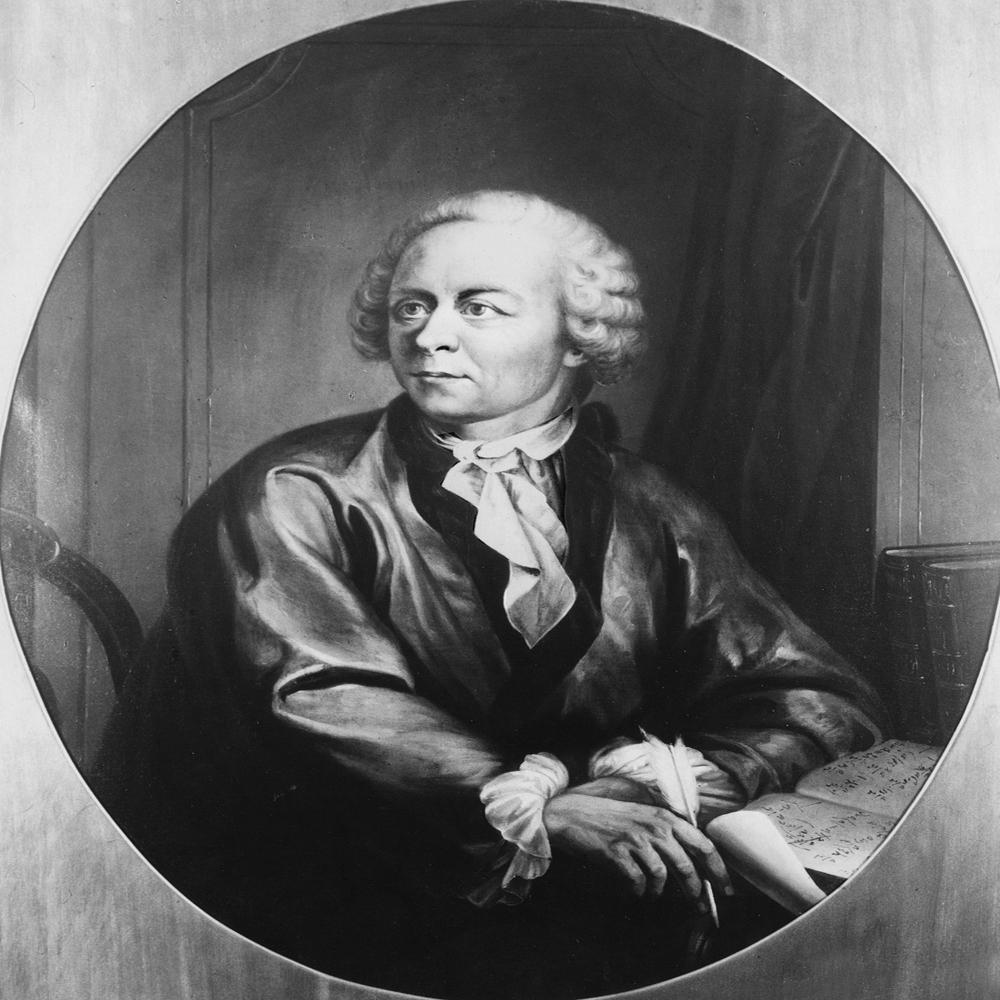
\includegraphics[width=\paperwidth]{euler (1).jpg}}; 
 % \end{tikzpicture}};
%\end{tikzpicture}





%\color{blue}
	\begin{center}
		\thispagestyle{empty}
		%\pagecolor{BrickRed}

\vspace*{1.5cm}

		{\Huge\textbf{DM me Your Answer!}}
		\vspace*{1cm}
	\end{center}
		
		{\Huge A positive integer $n $ is said to have property $P $ when for any number $a \in\mathbb {Z}^+$ if $n $ divides $a^n-1$ then $n^2$ also divides $a^n-1$. Prove that \begin{enumerate}
\item All primes have the property $P $
\item There are infinitely many composite numbers which have the property $P $
\end{enumerate}}
	\begin{center}	
		
		\vspace{1cm}

{\fontsize{40}{30}\selectfont 
		
		$$\boldsymbol{\sum \limits_{i=0}^{Creative} Math_i = Solving}$$}
		
		\vspace{1cm}
		
		\begin{mybox}\Huge{\begin{center}\textbf{\textcolor{Green4}{Solution $\to$}} \end{center}}\end{mybox}
	\end{center}
\end{document}
